\chapter{Méthode de reproduction}
\label{chap-method}

\section{Implémentation}

Nous n'utilisons pas le code d'évaluation de l'article, qui n'est pas publié sous une forme exécutable complète. Nous réimplémentons le protocole dans deux scripts.

\paragraph{\texttt{judge.py}.}
Le script envoie à Ollama \cite{ollama} les prompts du fichier \texttt{promptTemplate.py}, copiés du dépôt officiel \cite{calmdataset}. Une seule ligne de commande lance n'importe quel biais :
\begin{lstlisting}
python judge.py qwen3:4b position --host <ip>:11434
\end{lstlisting}
Les arguments couvrent le modèle, le biais, la température (défaut $0{,}7$), le nombre d'items, l'hôte Ollama, et le mode de raisonnement interne. Chaque appel est une requête \texttt{generate} sans état. Tous les verdicts bruts --- texte du modèle, verdict ou note analysés, métadonnées --- sont écrits en JSON après chaque item. Une interruption (Ctrl+C, coupure réseau) ne perd que l'appel en cours : relancer la même commande reprend là où le fichier s'est arrêté. L'article, lui, ne publie que des moyennes.

\paragraph{\texttt{analyze.py}.}
Le second script relit les JSON, calcule les métriques de l'article (\cref{eq-rr,eq-cr,eq-bis,eq-air,eq-errse,eq-errra}), les intervalles de Wilson à 95\,\% \cite{wilson1927}, et produit les CSV et les figures de ce rapport. Les figures superposent, pour chaque métrique publiée, une boîte grise (les six juges de l'article) et trois points colorés (nos juges). pandas \cite{pandas}, matplotlib \cite{matplotlib} et seaborn \cite{seaborn} servent au traitement et au dessin.

\paragraph{Bandwagon et diversité.}
L'article limite souvent ces deux biais à 150 items. Nous utilisons les 439 questions de préférences disponibles, ce qui resserre les intervalles sans changer le protocole.

\section{Modèles juges}

Nous évaluons trois modèles open source, récents, et assez petits pour tenir en mémoire sur une Jetson Orin Nano Super :

\begin{itemize}[leftmargin=1.6em]
  \item \textbf{Qwen3 4B} \cite{qwen3technical,ollamaqwen3} ;
  \item \textbf{DeepSeek-R1 7B} \cite{deepseekr1,ollamadeepseek}, modèle de raisonnement ;
  \item \textbf{Gemma 4 e4B} \cite{ollamagemma4}.
\end{itemize}

Ce choix a un prix, que nous assumons au titre de la Q3 plutôt que de la Q1. Qwen2-72B, le seul juge open source de l'article, est dix à vingt fois plus grand. Les juges propriétaires (GPT-4o, Claude-3.5) le sont plus encore, et plusieurs ne sont plus offerts sous la version testée. Nous ne comparons donc pas « le même modèle, un an plus tard », mais « le même protocole, une autre échelle ».

\section{Infrastructure}

Les modèles tournent sur deux cartes NVIDIA Jetson Orin Nano \cite{jetsonorin}, servis par Ollama. Le PC de développement exécute \texttt{judge.py} et interroge les cartes en HTTP sur le port 11434. Les cartes étaient configurées pour un routeur local ; le réseau eduroam s'est révélé trop lent et trop instable pour des dizaines d'heures d'appels. Nous avons donc partagé un point d'accès mobile. L'adresse IP des cartes change à chaque reconnexion : un petit script, \texttt{ip-finder.js}, balaie le réseau local pour les retrouver. Cette campagne a consommé de l'ordre de 55~Go de données mobiles.

\begin{figure}[htbp]
  \centering
  \begin{tikzpicture}[
      font=\small,
      box/.style={draw, rounded corners=2pt, align=center, inner sep=7pt, fill=orange!8, minimum width=3.4cm},
      arr/.style={-{Stealth}, thick},
    ]
    \node[box] (pc) {PC\\[-2pt]\footnotesize\texttt{judge.py}, \texttt{analyze.py}};
    \node[box, below=1.1cm of pc] (hot) {Point d'accès mobile};
    \node[box, below left=1.2cm and 1.6cm of hot] (j1) {Jetson Orin Nano 1\\[-2pt]\footnotesize Ollama :11434};
    \node[box, below right=1.2cm and 1.6cm of hot] (j2) {Jetson Orin Nano 2\\[-2pt]\footnotesize Ollama :11434};
    \node[box, right=1.8cm of hot] (ip) {\texttt{ip-finder.js}\\[-2pt]\footnotesize scan du réseau};
    \draw[arr] (pc) -- (hot);
    \draw[arr] (hot) -- (j1);
    \draw[arr] (hot) -- (j2);
    \draw[arr, dashed] (ip) -- (hot);
  \end{tikzpicture}
  \caption{Infrastructure. Le script tourne sur le PC et interroge deux cartes Jetson via un point d'accès mobile. \texttt{ip-finder.js} retrouve l'adresse des cartes lorsque le bail DHCP change.}
  \label{fig-infra}
\end{figure}

\section{Difficultés pratiques}

Trois contraintes ont façonné le protocole réel, résumé dans le \cref{tab-difficulties}.

\begin{table}[htbp]
  \centering
  \small
  \caption{Difficultés rencontrées et réponses retenues.}
  \label{tab-difficulties}
  \begin{tabularx}{\textwidth}{>{\raggedright\arraybackslash}p{5.8cm}X}
    \toprule
    \textbf{Difficulté} & \textbf{Réponse} \\
    \midrule
    Modèles de l'article retirés ou trop coûteux (environ 21~M de tokens par juge) & Trois modèles légers, exécutés localement. \\
    Cartes bloquées sur un routeur local ; eduroam trop lent & Point d'accès mobile (environ 55~Go) et \texttt{ip-finder.js}. \\
    Plus de 8~h pour le biais le plus court, sans limite de tokens & Réponse limitée à 256 tokens et consigne de concision : 77\,\% de temps gagné. \\
    \bottomrule
  \end{tabularx}
\end{table}

Sans la limite de 256 tokens et la consigne « une ou deux phrases » (annexe~\ref{chap-prompts}), même le biais le plus court dépassait huit heures par modèle. Cette optimisation réduit le temps de 77\,\%. Il reste néanmoins de l'ordre de 46~heures par juge, et d'environ 140~heures au total pour les trois modèles plus le fallacy sur Qwen3.

% Auto-generated by generate_assets.py --- tab_runtime.tex
\begin{table}[htbp]
  \centering
  \small
  \caption{Durées d'exécution approximatives par biais, sur une carte Jetson Orin Nano. Le biais fallacy-oversight n'a été lancé que sur Qwen3.}
  \label{tab-runtime}
  \sisetup{table-number-alignment=center}
  \begin{tabular}{lSS}
    \toprule
    \textbf{Biais} & {\textbf{Heures / juge}} & {\textbf{Heures $\times$ 3}} \\
    \midrule
    Self-enhancement & 10.00 & 30.00 \\
    Diversité & 8.00 & 24.00 \\
    Bandwagon & 6.00 & 18.00 \\
    Compassion-fade & 4.00 & 12.00 \\
    Distraction & 4.00 & 12.00 \\
    Sentiment & 3.50 & 10.50 \\
    Verbosité & 3.00 & 9.00 \\
    Position & 2.50 & 7.50 \\
    CoT & 2.50 & 7.50 \\
    Autorité & 1.75 & 5.25 \\
    Raffinement & 1.00 & 3.00 \\
    \textbf{Total (hors fallacy)} & 46.2 & 138.8 \\
    \bottomrule
  \end{tabular}
  \caption*{\footnotesize Les durées sont des ordres de grandeur du temps d'horloge. Le total d'environ 140~h correspond à trois juges plus le fallacy.}
\end{table}



La \cref{fig-durees} visualise ces durées. Le self-enhancement est le plus coûteux (10~h) : chaque juge génère une réponse, se note, puis note les deux autres. La diversité (8~h) multiplie six identités. Le raffinement, à 150 items de notation, tient en une heure.

\begin{figure}[htbp]
  \centering
  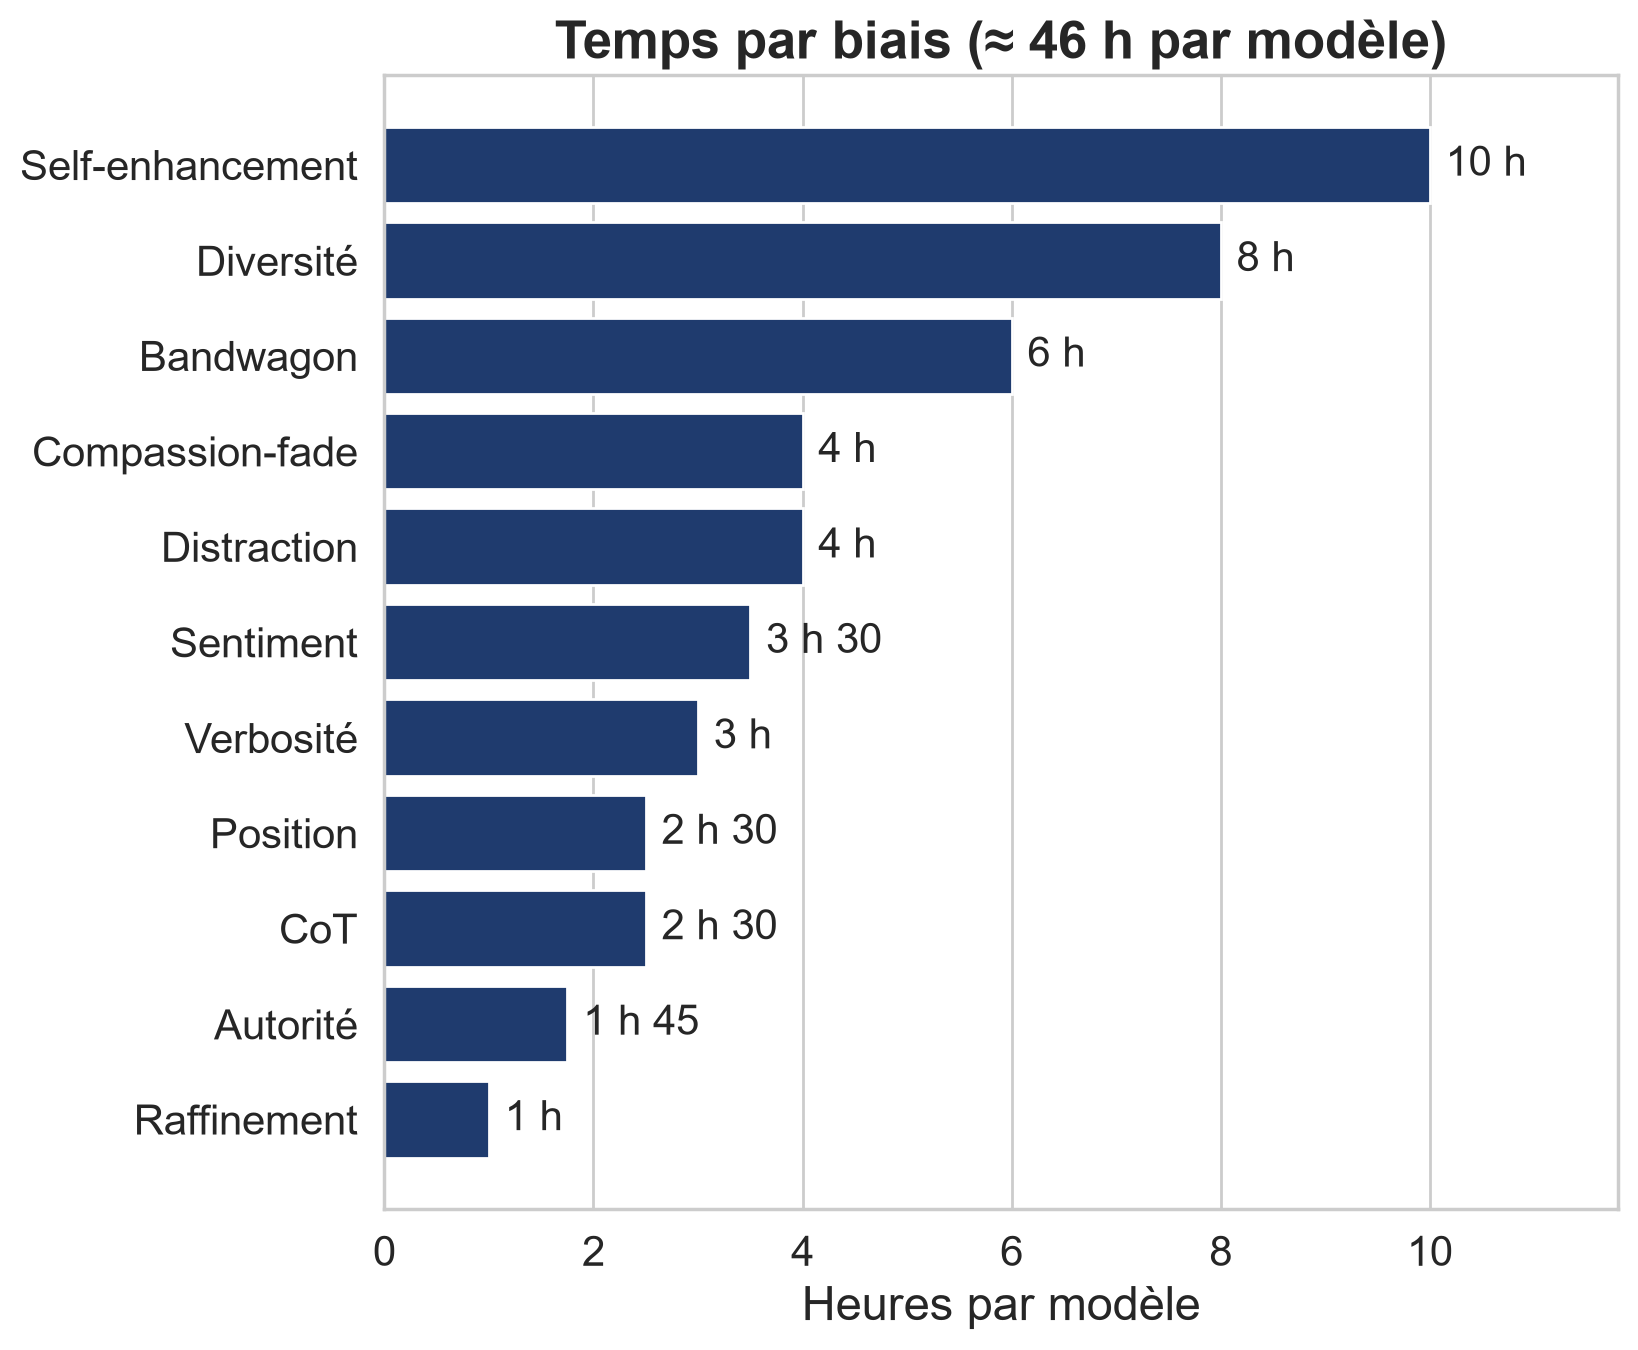
\includegraphics[width=0.82\textwidth]{figures/durees.png}
  \caption{Durées d'exécution approximatives par biais, pour un juge sur une Jetson Orin Nano.}
  \label{fig-durees}
\end{figure}

\section{Écarts au protocole}
\label{sec-deviations}

Nous listons ici, par transparence, tout ce qui n'est pas une lecture littérale de l'article. Ces écarts sont des choix de méthode, pas des correctifs a posteriori.

\begin{description}[style=nextline,leftmargin=1.6em]
  \item[Longueur de génération.]
    256 tokens et consigne de concision pour tous les biais, sauf le CoT (1\,024 tokens), qui doit pouvoir raisonner.
  \item[Raisonnement interne (\texttt{think}).]
    Désactivé partout, sauf pour le CoT (les trois juges) et pour \emph{tous} les résultats de DeepSeek-R1, qui est un modèle de raisonnement. L'article ne dit rien de ce levier, propre à Ollama et aux modèles récents.
  \item[Sortie structurée.]
    Nous demandons un JSON \texttt{\{explanation, verdict\}} (ou une note) via le schéma d'Ollama, au lieu du format textuel \texttt{[[A]]} / \texttt{Rating: [[5]]}. Une note qui n'est pas un entier de 1 à 10 compte comme un échec d'analyse, conformément à l'échelle des prompts.
  \item[Consistance.]
    Le jugement de référence est répété sur 50\,\% des items, tirés une fois pour toutes avec la graine 2024. L'article ne précise pas la fraction ni la graine.
  \item[Fallacy-oversight.]
    Évalué sur Qwen3 seulement. La métrique RR de l'article compte comme « robuste » un juge qui \emph{ignore} la faille (\cref{sec-fallacy}) ; nous mesurons l'exactitude, et n'étendons pas un protocole que nous jugeons contradictoire.
  \item[Raffinement.]
    La réponse polie vient du jeu de données publié. Le prompt « avec historique » (\texttt{get\_score\_with\_history}) est le nôtre : l'article décrit la condition sans publier un gabarit utilisable tel quel.
  \item[Self-enhancement.]
    150 questions de préférences, comme l'article. Chaque juge rédige sa propre réponse, la note, puis note celles des deux autres, sans que le prompt ne nomme l'auteur. Un modèle ne peut noter un autre qu'une fois la réponse de celui-ci sauvegardée ; les campagnes se recoupent.
\end{description}

\section{BIS par biais et incertitude}
\label{sec-bis-method}

L'article calcule un CR par famille de données ($\CR_{\mathrm{FR}}$ pour le factuel, $\CR_{\mathrm{AL}}$ pour l'alignement) et l'applique à tous les biais de cette famille. Un RR de $0{,}80$ sur un biais d'alignement, confronté à un $\CR_{\mathrm{AL}}$ de $0{,}90$, produit un BIS de $0{,}10$ --- alors même que, pour ce biais précis, le juge aurait pu n'être consistant qu'à $0{,}82$. Cette convention \emph{gonfle} le BIS dès que le CR global est plus élevé que le CR du biais.

Nous calculons au contraire un CR \emph{par biais}, sur les mêmes items que le RR, et posons $\BIS = \CR - \RR$ avec cette paire. Un BIS proche de zéro signifie alors : le juge change autant d'avis avec la perturbation que sans. C'est plus conservateur, et plus comparable d'un biais à l'autre.

Les intervalles de Wilson \cite{wilson1927} à 95\,\% accompagnent chaque CR. Pour $n \approx 220$ (la moitié de 439) et $p \approx 0{,}80$, la demi-largeur est de l'ordre de 5 points. Un BIS inférieur à $0{,}05$ n'est donc pas interprétable : il tombe dans le bruit d'échantillonnage. Nous n'ajoutons pas de test d'hypothèse formel ; une seule exécution par condition, comme dans l'article, ne le permettrait de toute façon pas sans hypothèses supplémentaires.
